% !TEX encoding = UTF-8 Unicode
%!TEX root = thesis.tex
% !TEX spellcheck = en-US
%%=========================================
\chapter{Introduction}

%%=========================================

\subsection*{Augmented Reality}

% (Jentoft, 2020) AR can be defined as a system that fulfills three basic features: a combination of real and virtual worlds, real-time interaction, and accurate 3D registration of virtual and real objects.

{
    \color{BrickRed}
    [TODO: Rewrite this shitty part]
    Augmented Reality (AR) describes the use of technology to insert computer generated three-dimensional visuals into the real world in real-time, and the ability to blend interaction between real-world and computer-based objects. 
}
Augmented Reality (AR) describes the use of computer technology to generate an audio-visual experience combining real-world impressions with computer generated graphics, and -essentially- the ability to interact seamlessly between both domains.
 

\noindent Ever since the infancy of AR technology, medical usage has been envisioned as a great potential. The idea of x-ray vision is seen both in science fiction and in genuine research dating all the way back to the 1930s when H. Steinhaus explored ways to visualize metal pieces inside the body \citep{Sielhorst2008}. There is now substantial interest in the use of AR within a wide array of medical fields as well as in industry and education. As an emerging technology there is still much research needed, and great leaps in hardware, software and sensor capabilities are bound to happen in the near future. Already AR shows promising results in both surgical settings and in education \citep{Singh2013}.

\subsection*{Neuroanatomy}

The study of neuroanatomy is concerned with the structural organization of the nervous system. This primarily means the brain and its structures, and that is what this project will focus exclusively on.
Within the study of neuroanatomy, the use of macroscopical brain dissections have long been the conventual practice for teaching the organization of the structures in the brain. Requiring cadavers and the single use of their brain, this method is highly resource intensive and has limited scalability. In addition, there are deeply concerning ethical problems with the use of animals in research. 

\section{Problem Formulation}

%%=========================================
\section{Motivation}

In light of the problems with physical brain dissections it is natural that the use of digital tools, three-dimensional modeling and visualization has been seeing growing use for educational purposes. 
%%=========================================
%%=========================================
According to \citep{Dalgarno2010} computer-aided learning generally increases understanding for anatomy. As anatomy in general, and neuroanatomy specifically are highly complex domains both visually and spatially, the ability to use the human senses in a real-world setting could result in greater intuition and understanding. With that in mind the use of augmented reality could be a natural way to virtualize the experience of a brain dissection, and further the unique capabilities of AR could enable innovative ways of learning. \citep{Moro2017} shows the possibility of greater immersion and engagement while using augmented reality in teaching anatomy to medical students. This has also recently been shown with promising result by  \citep{Wish2020}, where COVID-lockdown required from-home teaching, and the use of HoloAnatomy, an anatomy application for the HoloLens, performed significantly better than even conventional in-class lectures.

%%=========================================
The main problem with most academic implementations, like \citep{Wish2020}, of AR in medical education is the use of head-mounted display (HMD) devices like the HoloLens 2 and Magic Leap, which in the near to mid-term future will have limited practical use in education, as a result of the high price-tag, combined with the still inadequate general use-case for these types of devices.
This project will try to mend these challenges by having the lecturer using an HMD and having student view and interact with the lecture in an AR-based application running on their smartphone. 
%%=========================================
This is possible because of the great leap in AR-performance seen in recent models of Android and especially iPhones, in combination with development platforms like \nameref{chap:unity}, \nameref{chap:mrtk} and \nameref{chap:photon} (see \autoref{chap:tools}) which enables multiplatform development and real-time collaboration between devices. 
% In this pursuit we will also make use of high-resolution 3D imagery of a rat brain (see \autoref{chap:ratbrain}).  
% %%=========================================
\todo[inline]{Introduce Nevrolens and WHS brain}
The aim of the project will be to create a seamless educational experience in Augmented Reality which can be valuable both on an HMD device and a modern smartphone. The focus will be on investigating its feasibility as an educational tool both in a lecture-type setting and for students to explore the brain anatomy independently. 

%%==========================================




%%=========================================
\subsection*{What Remains to be Done?}

%%=========================================
\section{Objectives / Research Questions}
What follow are the research questions which motivates this project: \\
\noindent
\textbf{Main RQ:} How can AR support teaching of rat brain anatomy and dissection for medical students?
\begin{itemize}
    \item {
        \textbf{Sub-RQ1:} How should interaction in be implemented in AR to accommodate medical professionals?
    }
    \item {
        \textbf{Sub-RQ2:} How will a collaborative experience shared between an HMD and a smartphone compare to accommodate medical professionals?
    }
    {
        \newline
        \color{BrickRed}
        \textbf{Sub-RQ3: }
        Something about macro + microscopic visualization, some suggestions:
        \item Can microscopical data seamlessly be integrated into a macroscopical model? 

        \item Can understanding be increased by integrating microscopical data into a macroscopical model?

        \item Will having integrated microscopical data in a macroscopical model lead to greater understanding?
    }
\end{itemize}


%%=========================================
\section{Approach}


\subsection*{Research method}

\begin{wrapfigure}{R}{0.50\textwidth}
    \begin{center}
        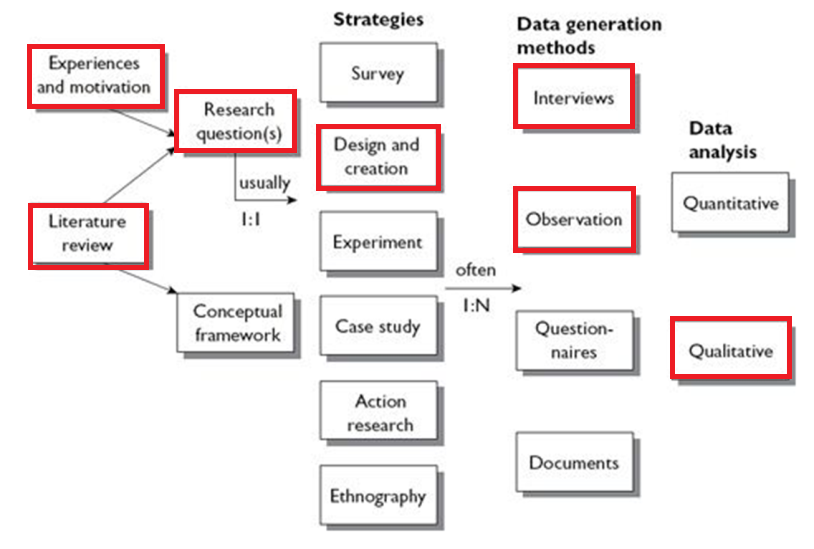
\includegraphics[width=0.42\textwidth]{fig/researchplan_image}
    \end{center}
    \caption{Model of the research process as illustrated in \citet{oates2006} }
    \label{researchplan_img}
\end{wrapfigure}

The research questions were derived through discussing the needs of the intended users with neuroscientists at the Kavli Institute. It was then narrowed down by a literature review, finding a lack of satisfactory substitutions for real brain dissections and especially finding no attempt at a practical multiplatform application for a more scalable use for students. The projects research question falls under the strategy of Design and Creation as the main goal is to develop a useful application for medical education. The focus on a smartphone solution was further motivated by the COVID-pandemic making from-home learning quite essential and making the passing around of HMD devices an unwanted scenario. As part of an agile software development model the gathering of qualitative data from observations and interviews within the scope of user testing will be essential. 

\subsection*{Development method}

\section{Contributions}
%% write about macro vs micro stuff

The research product resulting from this project will be a new computer-based software application using augmented reality and running on multiple platforms like HoloLens 1 and 2, Android and more. The aim will be to develop an application that can bridge the gap between expensive head mounted displays and everyday smartphones which you will find in the pocket of any student, and to use this as a collaborative tool for learning neuroanatomy. Throughout the development period we will consult with medical professionals and gather feedback from students on the usability of the application.

{
    \color{BrickRed}
    \noindent
    \newline
    Something about macro + micro
}

%%=========================================
\section{Limitations}

%%=========================================
\section{Outline}

